\chapter{Réalisation}
\label{chap:realisation}

\section*{Introduction}
\addcontentsline{toc}{section}{Introduction}

Ce chapitre détaille la phase de réalisation du projet, organisée en six sprints de deux semaines (cf. \cref{tab:planification}). Pour chaque sprint sont présentés les objectifs, le contenu livré et, le cas échéant, les difficultés rencontrées.

\section{Sprint 1 -- Fondations et infrastructure}

\subsection*{Objectifs}
Mettre en place l'environnement de développement conteneurisé, le socle de données du domaine, et la connexion en lecture au catalogue PrestaShop.

\subsection*{Réalisation}

Le sprint a débuté par la mise en place de l'\textbf{infrastructure Docker Compose} regroupant l'ensemble des services de la plateforme (\emph{ai-core}, backoffice, PostgreSQL, Redis, ChromaDB, Prometheus, Grafana), ainsi que le pipeline d'\textbf{intégration continue} sur GitHub Actions et les \textbf{migrations Alembic} versionnant le schéma de base de données.

Les \textbf{modèles de données du domaine} ont été implémentés : \texttt{Tenant} (isolation multi-tenant), \texttt{Conversation} et \texttt{Message} (historique du chat), \texttt{Product} (catalogue) et \texttt{Coupon}. La configuration PostgreSQL a été durcie (variables d'environnement sécurisées, taille de pool de connexions configurable, \emph{healthchecks} de conteneur).

Enfin, un \textbf{client PrestaShop asynchrone} a été développé (couvert par 33 tests unitaires), ainsi qu'un \textbf{service de synchronisation de catalogue} multi-tenant réalisant un \emph{upsert} en masse des produits, avec indexation vers ChromaDB optimisée par pagination en flux continu et évitement des ré-indexations inutiles par comparaison de hachage de contenu.

\section{Sprint 2 -- Moteur de chat IA}

\subsection*{Objectifs}
Livrer le c\oe{}ur fonctionnel du chat conversationnel : recherche augmentée par récupération de contexte (RAG) et orchestration de bout en bout de la réponse.

\subsection*{Réalisation}

La \textbf{recherche vectorielle de produits} (RAG) a été intégrée à l'endpoint de chat, avec prise en charge du contexte multi-tenant et repli explicite (réponse générique, sans blocage) lorsque la recherche ne retourne aucun résultat pertinent. Le patron \textbf{Unit of Work} a été mis en place pour garantir qu'une conversation entière (persistance du message utilisateur, de la réponse, des métadonnées associées) s'exécute dans une transaction cohérente. Le service d'orchestration du chat (\texttt{ChatService}) a été finalisé avec une logique d'idempotence permettant de court-circuiter le traitement d'une requête déjà traitée, ainsi que des garanties de sécurité vis-à-vis des accès concurrents sur une même conversation.

\section{Sprint 3 -- Sécurité, multi-tenance et supervision}

\subsection*{Objectifs}
Fiabiliser la plateforme avant montée en charge réelle : sécurité applicative, isolation multi-tenant, observabilité, et correction des dysfonctionnements découverts lors des tests d'intégration approfondis.

\subsection*{Réalisation}

Ce sprint a été marqué par la découverte, via des tests d'intégration plus poussés que ceux existants jusqu'alors, de plusieurs écarts significatifs entre le comportement attendu du système et son comportement réel :

\begin{itemize}
    \item les \textbf{garde-fous de sécurité} (\texttt{GuardrailsOrchestrator}, détection d'injection de prompt, masquage de données personnelles) existaient dans le code mais n'étaient \textbf{pas effectivement appelés} par l'endpoint de chat en production -- ils ont été câblés dans le chemin réel de traitement d'un message ;
    \item la \textbf{limitation de débit} (\emph{rate limiting}) était silencieusement désactivée sur l'ensemble des routes ;
    \item l'\textbf{authentification par clé API} des tenants ne fonctionnait pas de bout en bout et a dû être corrigée pour être réellement opérante ;
    \item une \textbf{faille de contournement d'authentification} a été identifiée dans le middleware de résolution du tenant et corrigée en priorité ;
    \item la \textbf{persistance des conversations et des messages}, pourtant présente dans le code depuis le sprint 2, ne s'exécutait en réalité jamais dans certains chemins -- aucune conversation n'était donc durablement enregistrée. Le défaut a été isolé et corrigé, de même que plusieurs points d'entrée laissés à l'état d'ébauche (historique de conversation, retour utilisateur, clôture de conversation).
\end{itemize}

Ces corrections, bien que non prévues telles quelles dans le backlog initial, ont été traitées en priorité dès leur découverte : elles conditionnaient la fiabilité de toute fonctionnalité construite par la suite. Le sprint s'est conclu par la mise en place du \textbf{supervisionnement applicatif} (métriques Prometheus, tableaux de bord Grafana), la correction de plusieurs métriques instrumentées mais jamais alimentées (compteurs de coût et de tokens du modèle de langage, score de confiance des réponses, panneaux d'alerte affichant systématiquement l'absence de donnée), ainsi que par la résolution de treize vulnérabilités logicielles (CVE) détectées par l'analyse de dépendances, et la mise en place d'une analyse de qualité de code continue (SonarCloud).

\section{Sprint 4 -- Backoffice Laravel/Filament : socle}

\subsection*{Objectifs}
Construire le socle du backoffice d'administration : structure de l'application Filament, client REST vers l'API \emph{ai-core}, premières pages d'administration.

\subsection*{Réalisation}

L'application \textbf{Laravel 13 / Filament 3} a été initialisée, avec un client REST dédié (\texttt{AiCoreClient}) constituant le \textbf{seul point d'accès} du backoffice vers l'API \emph{ai-core} -- aucune autre classe de l'application n'effectue d'appel HTTP direct vers ce service, ce qui centralise la gestion des erreurs réseau et la dégradation en cas d'indisponibilité. Un premier tableau de bord et une première version de la page \emph{Agent IA Admin} ont été livrés, ainsi qu'une page de paramétrage du tenant.

L'intégration avec PrestaShop a été complétée côté marchand par un \textbf{module réel} embarquant un widget de chat IA directement sur le site marchand. Plusieurs anomalies bloquantes ont été corrigées pendant ce sprint, notamment un \textbf{scénario de verrouillage total et systématique} du panneau d'administration (l'administrateur perdait l'accès au backoffice dans une situation reproductible à 100~\%), des erreurs HTTP 403 intermittentes liées à la configuration de session, ainsi que l'activation du mode \emph{WAL} de SQLite pour supporter des accès concurrents lors des tests automatisés.

\section{Sprint 5 -- Moteur de règles et agent IA d'administration sécurisé}

\subsection*{Objectifs}
Livrer les deux fonctionnalités centrales du stage : le moteur de règles métier permettant de configurer le chat sans redéploiement, et la refonte de l'agent IA d'administration sur des bases réelles et sécurisées.

\subsection*{Réalisation}

\paragraph{Moteur de règles.} Le modèle \texttt{Rule}, préexistant dans le schéma de base de données mais jamais exploité, a été relié au flux de traitement du chat. L'évaluation des règles (\texttt{RuleEvaluator}) a été implémentée comme une fonction pure, testée unitairement de façon exhaustive (voir \cref{chap:tests}), puis intégrée dans l'endpoint de chat juste après la classification d'intention : en cas de correspondance, l'action associée (réponse préétablie, instruction injectée, génération de coupon) est appliquée selon le mécanisme détaillé à la \cref{fig:rules-flow}. Une interface complète de gestion des règles (création, modification, suppression) a été exposée côté API puis côté backoffice. La politique de remise historiquement codée en dur dans le service de coupons a été repliée dans ce même mécanisme de règles, avec conservation d'une valeur par défaut en l'absence de règle applicable.

\begin{figure}[h]
    \centering
    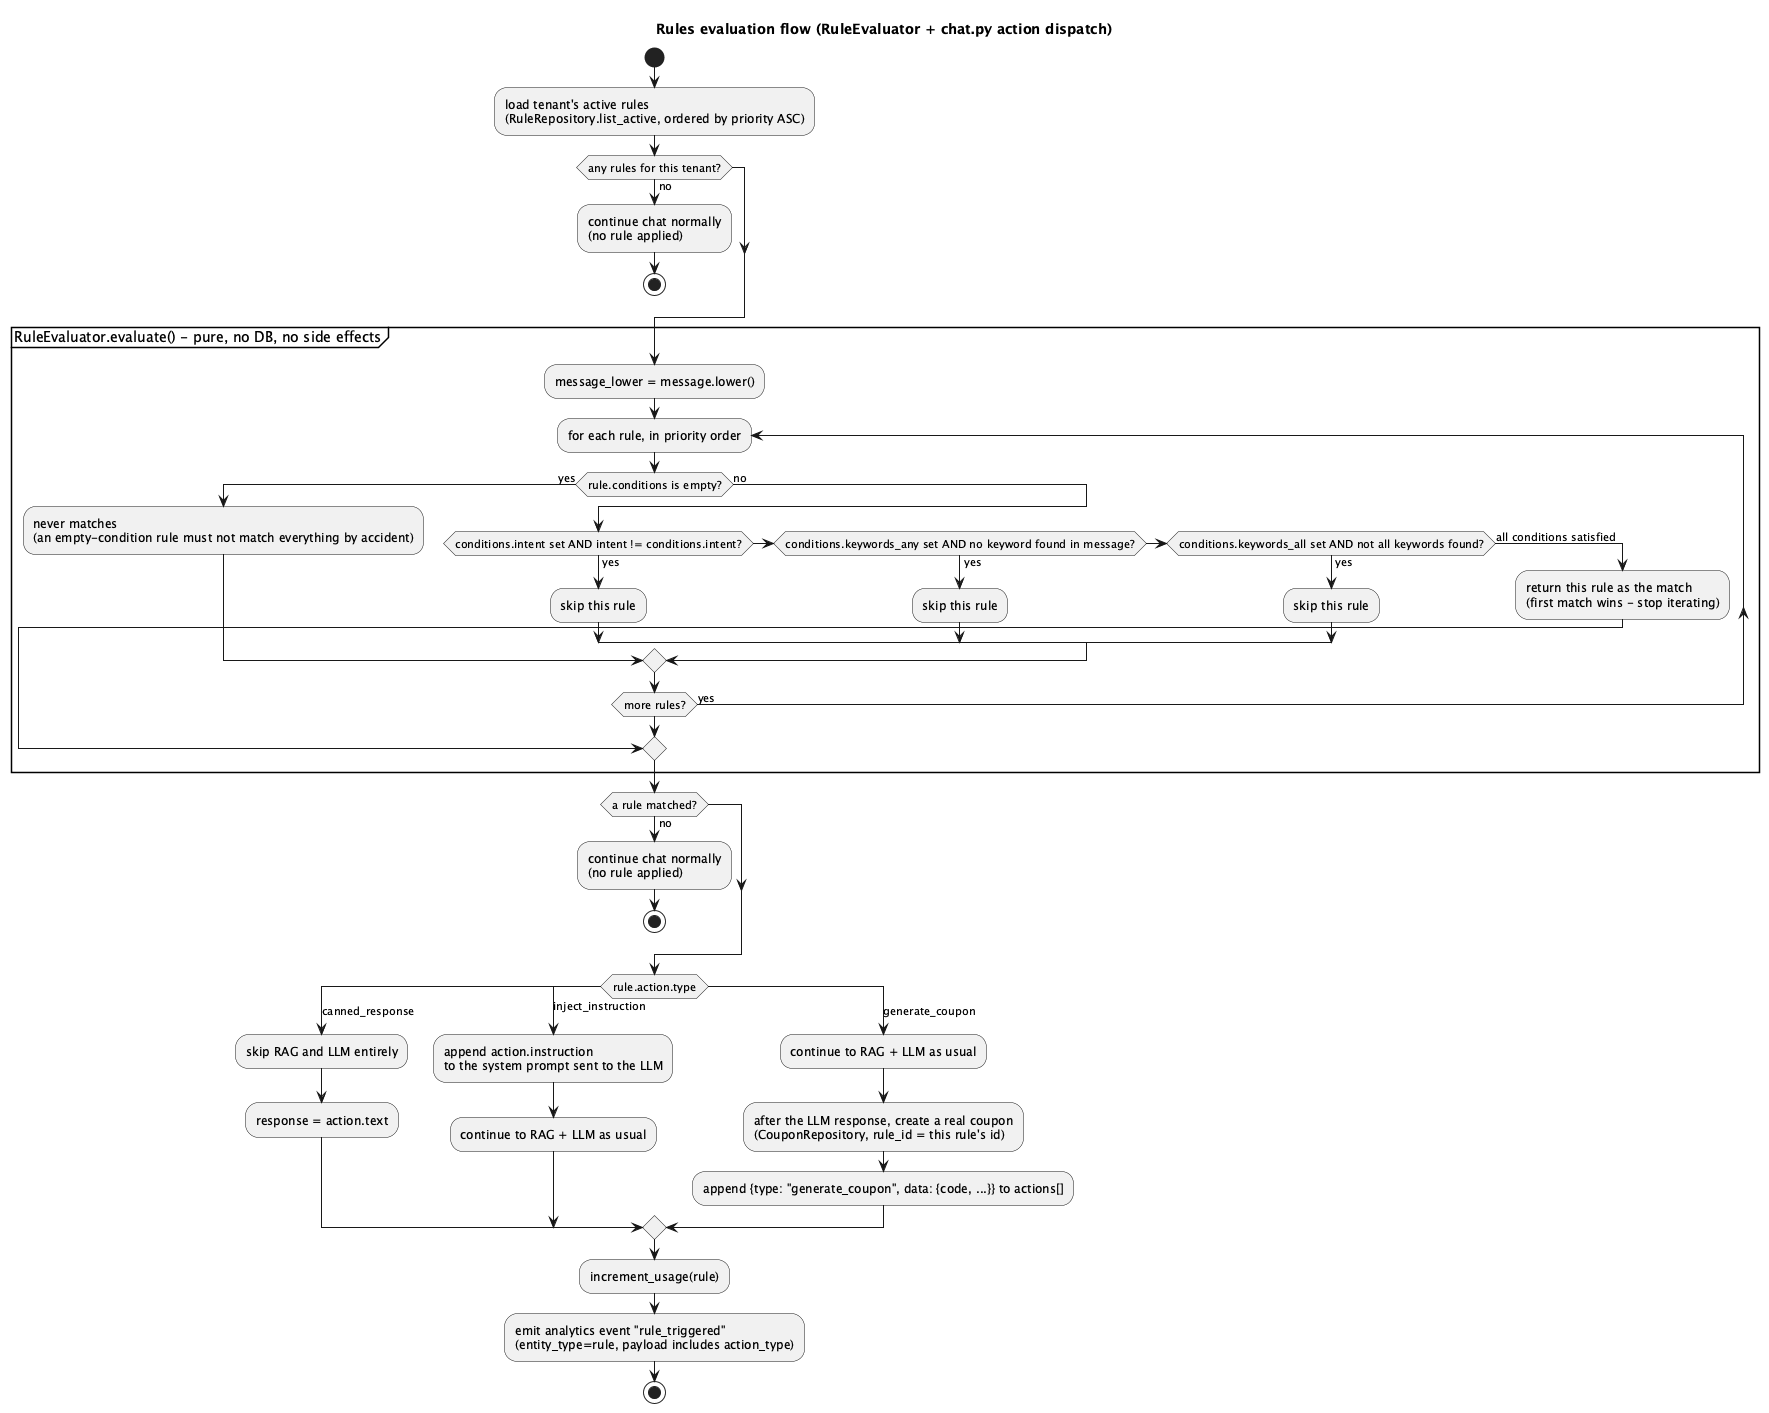
\includegraphics[width=0.9\textwidth]{../diagrams/Rules_Evaluation_Flow.png}
    \caption{Diagramme d'activités : évaluation des règles et répartition des actions}
    \label{fig:rules-flow}
\end{figure}

\paragraph{Agent IA d'administration.} Conformément au choix de conception exposé au \cref{chap:conception}, l'agent d'administration a été entièrement reconstruit. Un analyseur de commandes (\texttt{AdminCommandParser}) restreint désormais l'agent à un ensemble fermé d'actions prédéfinies, qu'elles soient exprimées de façon structurée ou en langage naturel (classification par mots-clés). Le système de sécurité (\texttt{AdminAISafetySystem}) a été effectivement adossé à Redis -- corrigeant un écart entre la documentation du composant, qui annonçait un état persistant, et son implémentation réelle, qui le maintenait jusque-là en mémoire locale du processus.

Les données présentées par l'agent (statistiques, produits en demande, demande non satisfaite) ont été entièrement reconstruites à partir du nouveau service \texttt{InsightsService}, remplaçant des valeurs d'exemple fixes (chiffre d'affaires fictif, noms de produits génériques) par des agrégats calculés sur les messages, conversations, produits et coupons réellement enregistrés. Un défaut a été détecté lors des essais manuels de l'interface d'administration reconstruite : les paramètres saisis via le formulaire du backoffice étant systématiquement transmis sous forme de chaînes de caractères, une comparaison numérique effectuée lors de la simulation d'une action (\emph{dry-run}) provoquait une erreur de type non gérée. Ce défaut a été corrigé par une coercition défensive des paramètres numériques, et une régression a été ajoutée à la suite de tests pour empêcher sa réintroduction.

\section{Sprint 6 -- Finalisation du backoffice et documentation}

\subsection*{Objectifs}
Achever l'exposition, côté backoffice, des fonctionnalités livrées au sprint précédent, et mettre à jour la documentation du projet en fin de stage.

\subsection*{Réalisation}

Le tableau de bord du backoffice a été doté de \textbf{graphiques réels} (Chart.js), alimentés par un nouvel endpoint d'API dédié aux séries temporelles, remplaçant les graphiques statiques initiaux. Une page \emph{Coûts \& Messages} a été ajoutée pour le suivi de la consommation du modèle de langage (tokens, coût, latence moyenne, messages les plus coûteux), ainsi qu'un navigateur de conversations permettant de consulter l'historique complet des échanges d'un tenant, et une page \emph{Insights} restituant l'ensemble des indicateurs de demande calculés par le service dédié.

L'interface de l'agent IA d'administration, jugée initialement trop rudimentaire (un simple formulaire de sélection d'action), a été retravaillée en une véritable \textbf{interface de type conversation}, conservant l'historique des échanges dans la session et présentant chaque résultat (statistiques, propositions de stratégie marketing, codes de coupons générés) sous une forme visuelle adaptée à sa nature plutôt qu'en JSON brut. Un défaut d'expérience utilisateur a également été corrigé sur les graphiques de répartition des intentions : en l'absence de toute donnée sur la période sélectionnée, un graphique vide s'affichait sans distinction visuelle avec un graphique en échec technique ; un état vide explicite a été introduit.

Le sprint s'est conclu par la consolidation de la documentation du projet : réécriture du \texttt{README}, mise à jour des diagrammes d'architecture pour refléter le système effectivement livré plutôt que sa conception initiale, et export automatisé du schéma \texttt{OpenAPI} de l'API depuis l'application elle-même, garantissant sa cohérence avec le code réel.

\section*{Conclusion}
\addcontentsline{toc}{section}{Conclusion}

Ce chapitre a détaillé, sprint par sprint, la réalisation du projet. Le chapitre suivant présente la démarche de tests et de validation mise en \oe{}uvre pour garantir la fiabilité de l'ensemble.
